\documentclass[../../Thesis.tex]{subfiles}
\begin{document}
\header{Data}
The dataset we used for this research consists of all articles\footnote{From Elseviers corpus} published in 2017 which have been published in a journal that has, in 2017, atleast 150 publications. This results in a total dataset of $1.391.543$ articles from $3.759$ journals.
\begin{table}[hbt]
\begin{center}
\begin{tabular}{|l|c|c|c|c|}
\hline
 & Total word count & Unique word count & Total token count & Unique token count \\
\hline
Title & $18.822.399$ & $939.665$ & $14.742.192$ & $230.805$ \\
\hline
Abstract & $264.653.020$ & $5.853.077$ & $171.474.473$ & $738.961$ \\
\hline
Total & $283.475.419$ & $6.209.769$ & $186.962.354$ & $763.475$ \\
\hline
\end{tabular}
\end{center}
\caption{Corpus size}\label{table:corpusSize}
\end{table}\\
The word occurrences follow the pattern of a pareto distribution as described by~\citet{wiegand2018word}. This distribution is visualized in XXXXXX, which displays the occurrences of the first 2.000 tokens of the corpus.
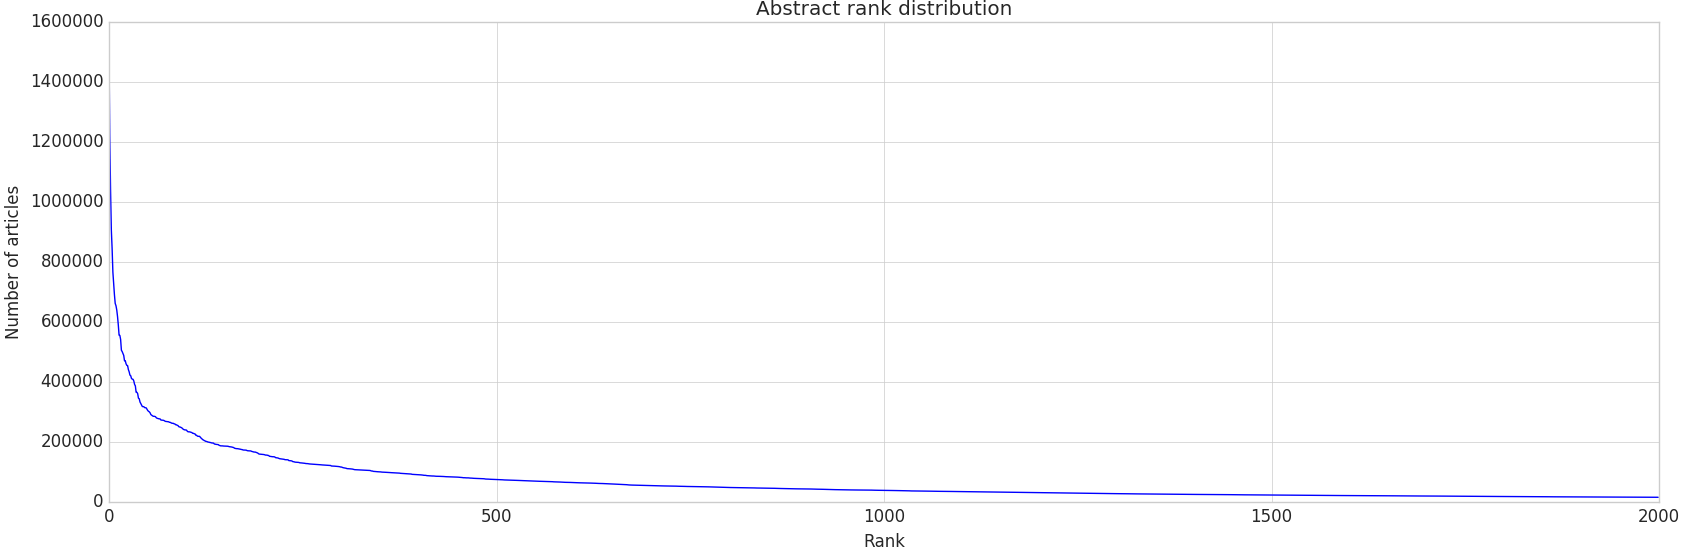
\includegraphics[width=6.5in]{Plots/word_occurrences}\\
\end{document}

% RAW DATA:
% 1,391,543 articles
% 14 811 433 title tokens			230805 unique		18.822.399			939.665
% 172 150 921 abstract tokens		738961 unique		264.653.020			5.853.077
% 186 962 354 total tokens			763475 unique		283.475.419			6.209.769
% 3,759 journals

% split = 79.9509609117 - 20.0490390883

% training numbers
% 10K = percentage?}